\documentclass[a4paper,12pt]{article}

\usepackage[utf8]{inputenc}
\usepackage{graphicx}
\usepackage[dvipsnames]{xcolor}

%\usepackage[defaultmono]{droidmono}

\usepackage{amsmath,amssymb,amsthm,textcomp}
\usepackage{enumerate}
\usepackage{multicol}
\usepackage{tikz}
\usepackage{listings}
%\usepackage{pst-plot}
\usepackage{geometry}
\usepackage{sidecap}
\geometry{total={210mm,297mm},
left=25mm,right=25mm,%
bindingoffset=0mm, top=20mm,bottom=20mm}


\linespread{1.3}

\newcommand{\linia}{\rule{\linewidth}{0.5pt}}

%\savedata{\data}[{{0,0},{1,1},{2,11},{3,6},{4,6},{5,3},{6,2},{7,0},{8,0},{9,1},{10,1},{11,0},{12,1},{13,0},{14,0},{15,0},{16,1},{17,1}}]

%\renewcommand\lstlistingname{Code}

\definecolor{backcolour}{rgb}{0.95,0.95,0.95}

\lstset{%
    backgroundcolor=\color{backcolour},
    basicstyle=\ttfamily\scriptsize,
    breaklines=true,
    captionpos=t,
    numbers=left,
    numberstyle=\tiny,
    numbersep=5pt,
    frame=tb,
    commentstyle=\color{PineGreen},
    keywordstyle=\color{RoyalBlue}
}

% custom theorems if needed
% my own titles
\makeatletter
\renewcommand{\maketitle} {%
\begin{center}
\vspace{2ex}
{\huge \textsc{\@title}}
\vspace{1ex}
\\
\linia\\
\@author \hfill \@date
\vspace{4ex}
\end{center}
}
\makeatother
%%%

% custom footers and headers
\usepackage{fancyhdr}
\pagestyle{fancy}
\lhead{}
\chead{}
\rhead{}
\lfoot{Complex Network \textbar Assignment 1}
\cfoot{}
\rfoot{15M54097 - Page \thepage}
\renewcommand{\headrulewidth}{0pt}
\renewcommand{\footrulewidth}{0pt}
%

% code listing settings
%%%----------%%%----------%%%----------%%%----------%%%

\newcommand*{\quoteTitle}[1]{{#1}\ignorespaces}%
\newenvironment{Quote}[1]{
    \medskip\par\noindent\quoteTitle{#1}
    \par\noindent
    \begin{quote}
    }{
    \end{quote}
    \par\noindent\ignorespacesafterend
}

\newtheorem{theorem}{Theorem}

\begin{document}
\bibliographystyle{acm}
\title{Complex Network - Assignment 1}

\author{NGUYEN T. Hoang - SID: 15M54097}

\date{Fall 2015, W833 Mon. Period 5-6 \\ \hfill Due date: 2015/11/30}

\maketitle

\vfill
\section*{Problem}
\noindent
\begin{enumerate}
    \item Visualize the network of Zachary's karate club. (GML file is available at http://www-personal.umich.edu/~mejn/netdata/).
    \item Select two central vertices. Why do you think they are central?
    \item Show the diameter, density, average path length, and clustering coefficient of the (undirected) network.
    \item Draw a degree distribution (a histogram of the degrees of vertices) of the network.
    \item Select two vertices whose PageRank values are the highest.
    \item Divide the network into small groups and answer its modularity.
\end{enumerate}
\vfill
\pagebreak
\section*{Answer}
\noindent
\paragraph{1.} Zachary's karate club undirected network is visualized using Gephi \cite{gephi}. The nodes in the graph are labeled by its id in the GML file, and they are also colored by the node degree (deeper blue indicates higher node degree).

\begin{figure}[h]
    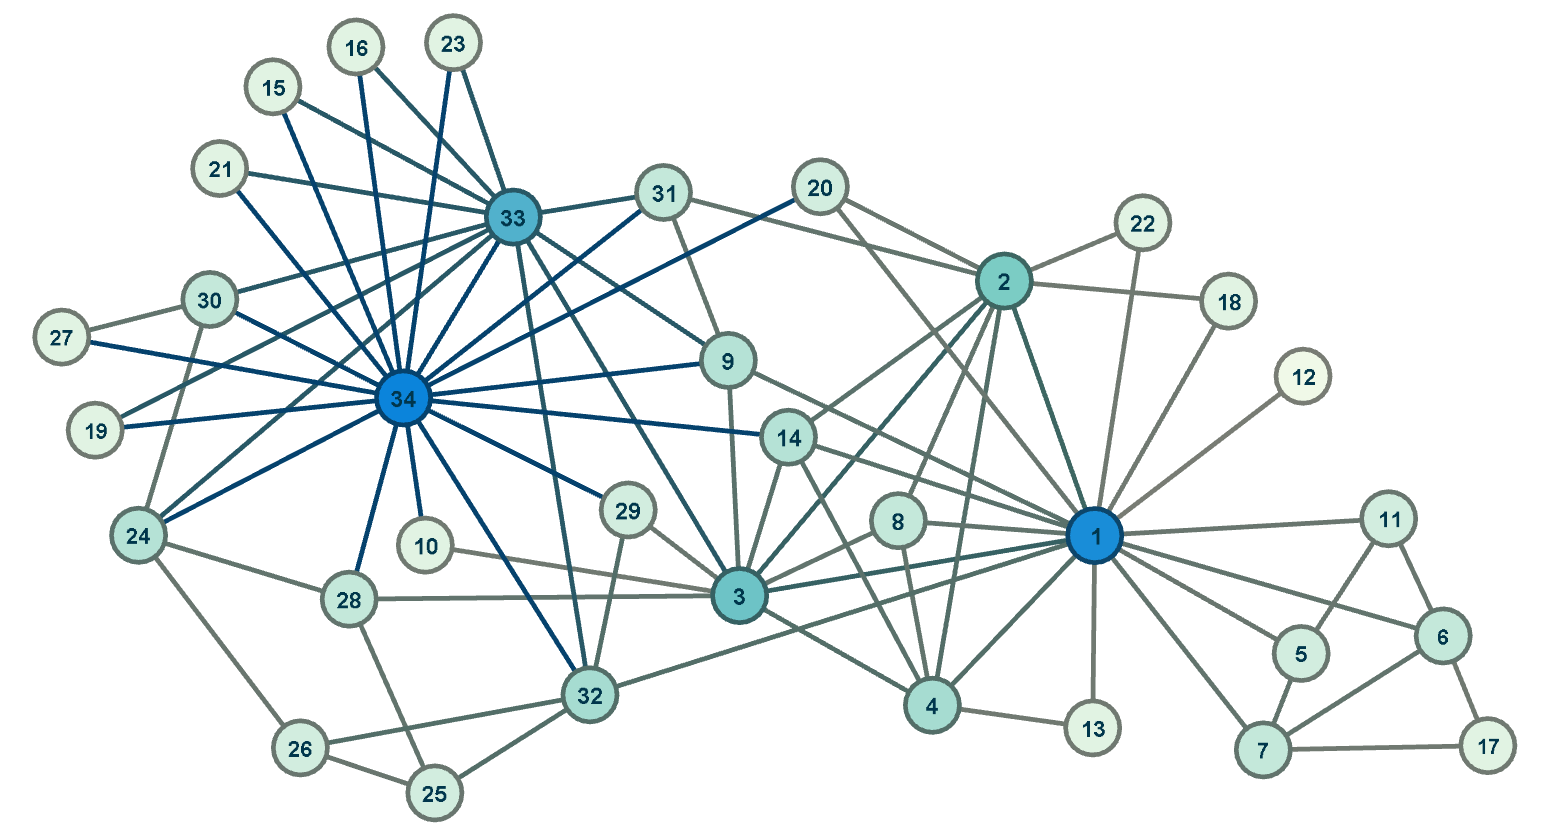
\includegraphics[width=\textwidth]{karate_viz.PNG}
    \caption{\emph{Visualization of Zachary's karate club network. Layout: Yifan Hu. Colored by edge degree.}}
    \label{fig:net}
\end{figure}

\paragraph{2.} Figure~\ref{fig:net} shows that there is two nodes with highest degree: \textbf{node 1} and \textbf{node 34}. I think that in term of \emph{intuitive centrality}, node 1 and node 34 are the top-2 most central nodes. In the network, node 1 and node 34 have the highest number of connection to other nodes. By observation, we can also see that any other nodes in the network must have a direct connection to node 1 or node 34. Therefore, the two most central nodes in the
network are node 1 and node 34. 

\begin{lstlisting}[language=Python, caption={Create the graph in SNAP.PY and print top-k highest degree centrality node.}]
 # Extracted from UnweightedUndirectedGraph class - File: get_data.py
 ...
 self._graph = snap.LoadEdgeList(snap.PUNGraph, edge_list_file, 0, 1, ' ')
 ...
 # Get the degree list 
 DegreeCentr = {}
 for NI in self._graph.Nodes():
   deg = snap.GetDegreeCentr(self._graph, NI.GetId())
   DegreeCentr[NI.GetId()] = deg
 sorted_ranking = sorted(ranking.items(), key=operator.itemgetter(1), reverse=True)
 return sorted_ranking[0:1]
\end{lstlisting}

\paragraph{3.} The metrics of the given network is summarized as below: \cite{mgit}
\begin{itemize}
        \setlength{\parskip}{0cm}
    \item Diameter of the network: 5
    \item Density: $\approx$ 0.14
    \item Average path length: $\approx$ 2.41
    \item Clustering coefficient: $\approx$ 0.57
\end{itemize}

\begin{lstlisting}[language=Python, caption={Graph metrics properties in SNAP.PY}]
 ...
 # Create a container for the graph
 karate_graph = UnweightedUndirectedGraph(edge_list, 'karate')
 ...
 # Python CLI 
 >>> karate_graph.approx_diameter(20) # 20 is number of sample
 5
 >>> graph.density 
 0.13903743315508021
 >>> graph.avg_path_length
 2.408199643493761
 >>> graph.get_quick_clust_coeff()
 0.5706384782076823
\end{lstlisting}

\paragraph{4.} The graph degree distribution visualization is obtained by creating frequency value \emph{csv} file and plot with Google Spreadsheet. 
\begin{figure}[h]
    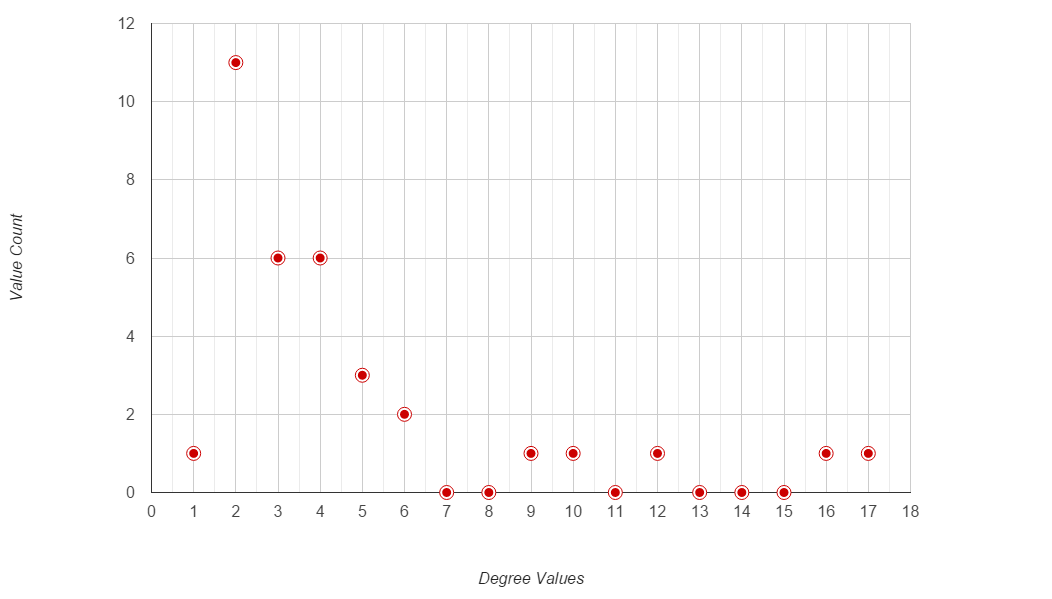
\includegraphics[width=\textwidth]{degree_dist.PNG}
    \caption{\emph{Degree distribution in the Zachary's Karate network.}}
    \label{fig:dist}
\end{figure} \\ 
The highest degree value in the network is 17 (1 node) and the lowest value is 1 (1 node). The most frequent degree value in the network is 2 with 11 nodes. For a social network in a sport club setting, I believe this distribution is natural.
\paragraph{5.} Two vertices with the highest PageRank values are: \cite{mgit}
\begin{itemize}
    \item Node 34 - PageRank value $\approx$ 0.100
    \item Node 1\ - PageRank value $\approx$ 0.097
\end{itemize}
\begin{lstlisting}[language=Python, caption={Graph PageRank calculation}]
 # Python CLI 
 >>> pr_dict_sorted = karate_graph.rank_pagerank()
 >>> pr_dict_sorted[0] # 0 is the highest score PageRank
 (34, 0.10091876156358327)
 >>> pr_dict_sorted[1] # 1 is the second highest score PageRank
 (1, 0.09700636750128044)
\end{lstlisting}

\paragraph{6.} I ran the Girvan-Newman community detection algorithm with resolution 1.0 and 2.0 to obtain 2 different graph partitionings as in figure~\ref{fig:m1} and figure~\ref{fig:m2}.
\begin{SCfigure}[\sidecaptionrelwidth][h]
    \centering
    \caption{\emph{Girvan-Newman community output. Resolution = 1.0. \textbf{Modularity} = \textbf{0.415}}\vspace{4em}}
    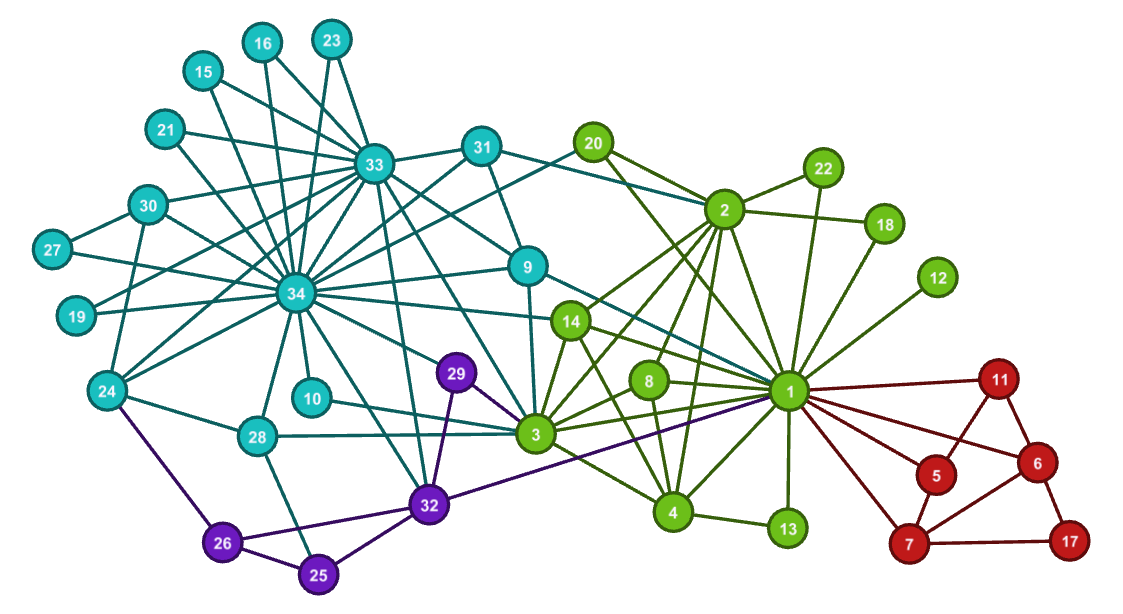
\includegraphics[width=0.6\textwidth]{subset_1.PNG}
    \label{fig:m1}
\end{SCfigure} 
\begin{SCfigure}[\sidecaptionrelwidth][h]
    \centering
    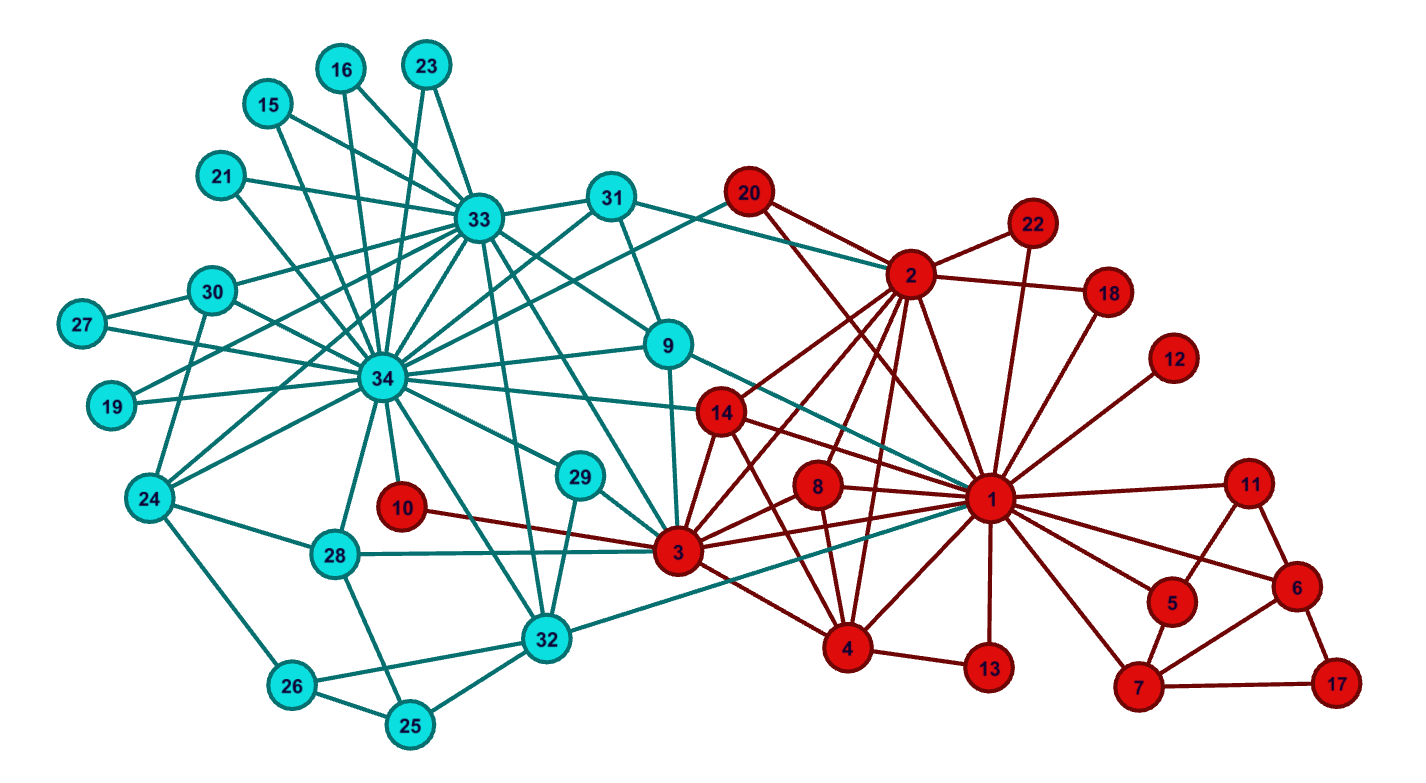
\includegraphics[width=0.6\textwidth]{subset_2.PNG}
    \caption{\emph{Girvan-Newman community output. Resolution = 2.0. \textbf{Modularity} = \textbf{0.371}}\vspace{4em}}
    \label{fig:m2}
\end{SCfigure} 


\bibliography{cn_a1}


\end{document}
